\documentclass[../NDCNNAI_main.tex]{subfiles}
\graphicspath{{\subfix{../fig/}}}

\begin{document}
	\subsection{Модель перцептрона}
	Обратимся подробнее к устройству перцептрона.
	Он, подобно биологическому нейрону состоит из следующих компонент:	
	\begin{itemize}
		\item Входных данных $x_1,\dots, x_n \in \mathbb{R}$ (синаптических сигналов), действие которых обусловлено переменными весами $w_1,\dots,w_n \in \mathbb{R}$ (синаптические силы).
		\item Мембранного потенциала (аффинная предактивационная функция):
		$$ V(x) = \sum_{i=1}^{n}w_ix_i + b = \langle w, x \rangle + b,$$
		где $b$ --- смещение. Оно может быть представлено в качестве веса $w_0$ с введением дополнительного входа $x_0 = 1$.
		\item Активационной функции ("<всё или ничего">, функция Хевисайда):
		$$ \sigma (V) = 
		\begin{cases}
			1, & V > 0, \\
			0, & V \leq 0.
		\end{cases}
		$$
	\end{itemize}
	На рисунке ниже приведена его схема.
	\begin{figure}[!ht]
		\centering
		\begin{tikzpicture}[scale=1.0]
        % Нейрон
        \shade[ball color=blue!30] (0,0) circle (1.25cm);
        \node at (0,0) {$\sigma(\langle w,x\rangle + b)$};
        
        % Входы
        \draw[-{Stealth[length=5]}] (-3,1.5) -- (-1.2,0.4); \node[left] at (-3,1.5) {$x_1$}; \node[left] at (-1.7,1.25) {$w_1$};
        \draw[-{Stealth[length=5]}] (-3,0.5) -- (-1.25,0.1); \node[left] at (-3,0.5) {$x_2$}; \node[left] at (-1.8,0.5) {$w_2$};
        \draw[-{Stealth[length=5]}] (-3,-0.5) -- (-1.25,-0.1); \node[left] at (-3,-0.5) {$\dots$};
        \draw[-{Stealth[length=5]}] (-3,-1.5) -- (-1.2,-0.4); \node[left] at (-3,-1.5) {$x_n$}; \node[left] at (-1.6,-1.25) {$w_n$};
        
        % Выход
        \draw[-{Stealth[length=5]}] (1.25,0) -- (3,0); \node[right] at (3,0) {$y$};
    \end{tikzpicture}
		\caption{Модель перцептрона}
		\label{pic:perceptron}
	\end{figure}
	Геометрический смысл модели: граница принятия решений $\lbrace x\colon \langle w, x \rangle + b = 0 \rbrace$ является гиперплоскостью, выходные данные разделяют $\mathbb{R}^n$ на два замкнутых полупространства.
	
	Нетрудно обобщить понятие перцептрона, определив просто искусственный нейрон.
	\begin{definition}[Искусственный нейрон]
		Это отображение $x \mapsto \sigma(\langle w, x \rangle + b)$ с функцией активации $\sigma\colon \mathbb{R} \rightarrow \mathbb{R}$ (не обязательно разрывной), весами $w \in \mathbb{R}^d$ и смещением $b \in \mathbb{R}.$ 
	\end{definition}
	
	\begin{definition}[Ridge-функция]	
	Когда мы обозначаем смещение $b$ через $w_0$, определяем константу $x_0 = 1$, функция предактивации принимает вид:
	$$\langle w, x \rangle + b =  \sum_{i=0}^{n}w_ix_i.$$
	Результат можно рассматривать как функцию от $x \in \mathbb{R}^{n+1}$ вида $ x \mapsto \sigma(x \cdot w)$,	где $\sigma\colon \mathbb{R} \rightarrow \mathbb{R}$, а $x \cdot w$ --- евклидово скалярное произведение двух векторов.
	Такая функция в контексте теории аппроксимации называется \emph{гребневой регрессией (ridge-функцией)}.
	Такие функции обладают тем свойством, что они всегда постоянны на гиперплоскостях:
	$$ x \cdot w = c, \quad c \in \mathbb{R}.	$$	
\end{definition}
	
\subsection{Основные функции активации}
Для обобщения модели перцептрона, функция активации Хевисайда заменяется на другие.
Ниже представлены каноничные функции активации, начиная с самой функции Хевисайда. 

\begin{itemize}
	\item \emph{Функция Хевисайда} (Рис. \ref{pic:heaviside}) --- это разрывная функция на множестве вещественных чисел $\mathbb{R}$, определяется как
  $$ \sigma (x) = 
	\begin{cases}
		1, & x > 0, \\
		0, & x \leqslant 0.
	\end{cases}
	$$
	\item \emph{Функция знака} (Рис. \ref{pic:sign}) --- это кусочно-определенная функция на множестве вещественных чисел $\mathbb{R}$:
	$$ \sigma (x) = \mathrm{sgn}(x) = 
	\begin{cases}
		1, & x \geqslant 0, \\
		-1, & x < 0.
	\end{cases}
	$$	
	\item \emph{ReLU функция} (Рис. \ref{pic:relu}) --- это кусочно-определенная функция на множестве вещественных чисел $\mathbb{R}$:
	$$ \sigma (x) = \max\{0, x\} =
	\begin{cases}
		x, & x > 0, \\
		0, & x \leqslant 0.
	\end{cases}
	$$
		
	\begin{figure}[!ht]
		\centering
		\subfloat[Функция Хевисайда]
		{
		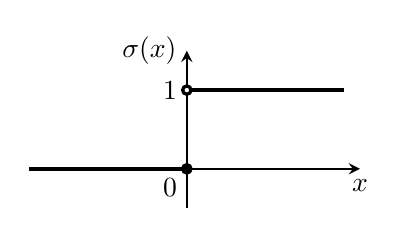
\begin{tikzpicture}[>=stealth, scale=1.0]
			% Оси
			\draw[->, thick] (-2,0) -- (2.2,0) node[below] {$x$};
			\draw[->, thick] (0,-0.5) -- (0,1.5) node[left] {$\sigma(x)$};

			% Подписи 0 и 1
			\node at (0,0) [below left] {$0$};
			\node at (0,1) [left] {$1$};

			\draw[very thick] (-2,0) -- (0,0);
			\draw[very thick] (0,1) -- (2,1);
			\draw[fill=white, draw=black, very thick] (0,1) circle (1.5pt);
			\draw[fill=black, draw=black, very thick] (0,0) circle (1.5pt);
		\end{tikzpicture}
		\label{pic:heaviside}
		}
		\hfill
		\subfloat[Функция знака]
		{
		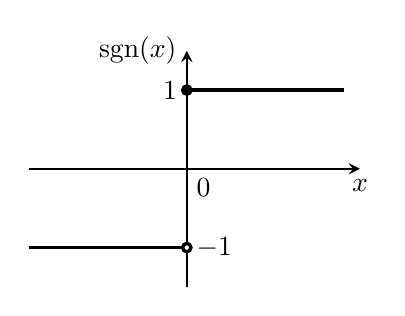
\begin{tikzpicture}[>=stealth, scale=1.0]
			% Оси
			\draw[->, thick] (-2,0) -- (2.2,0) node[below] {$x$};
			\draw[->, thick] (0,-1.5) -- (0,1.5) node[left] {$\mathrm{sgn}(x)$};

			% Подписи 0, 1 и -1
			\node at (0,0) [below right] {$0$};
			\node at (0,1) [left] {$1$};
			\node at (0,-1) [right] {$-1$};

			\draw[very thick] (-2,-1) -- (0,-1);
			\draw[very thick] (0,1) -- (2,1);
			\draw[fill=white, draw=black, very thick] (0,-1) circle (1.5pt);
			\draw[fill=black, draw=black, very thick] (0,1) circle (1.5pt);
		\end{tikzpicture}
		\label{pic:sign}
		}
		\hfill
		\subfloat[Функция ReLU]
		{
		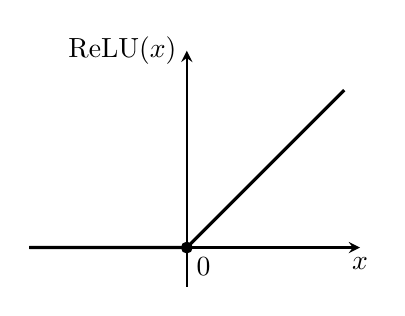
\begin{tikzpicture}[>=stealth, scale=1.0]
			% Оси
			\draw[->, thick] (-2,0) -- (2.2,0) node[below] {$x$};
			\draw[->, thick] (0,-0.5) -- (0,2.5) node[left] {$\mathrm{ReLU}(x)$};

			% Подписи 0 и 1
			\node at (0,0) [below right] {$0$};

			\draw[very thick] (-2,0) -- (0,0) -- (2,2);
			\draw[fill=black, draw=black, very thick] (0,0) circle (1.5pt);
		\end{tikzpicture}
		\label{pic:relu}
		}
		\caption{Кусочно-линейные функции активации}
	\end{figure}

	\item \emph{Логистическая сигмоида} (Рис. \ref{pic:sigmoid}) является гладким аналогом функции Хевисайда и задается формулой $ \sigma(x) = \frac{1}{1 + e^{-x}}$.
	
	\begin{figure}[!ht]
		\centering
		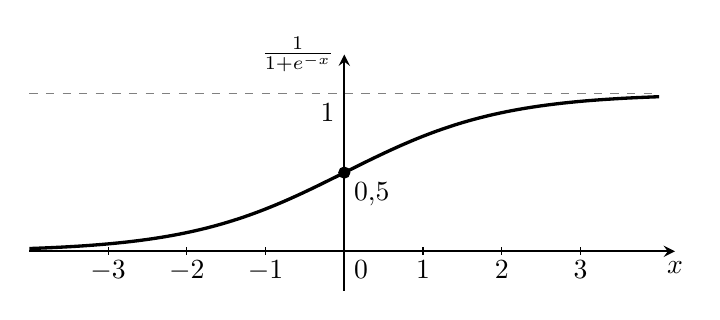
\begin{tikzpicture}[>=stealth, scale=1.0]
			% Оси
			\draw[->, thick] (-4,0) -- (4.2,0) node[below] {$x$};
			\draw[->, thick] (0,-0.5) -- (0,2.5) node[left] {$\frac{1}{1 + e^{-x}}$};

			% Деления на осях
			\foreach \x in {-3,-2,-1,1,2,3}
					\draw (\x,0.05) -- (\x,0) node[below] {$\x$} -- (\x,-0.05);
			\draw (0,0) node[below right] {$0$};
			\draw (0,1) node[below right] {$0,\!5$};
			\draw (0,2) node[below left] {$1$};

			\draw[dashed, gray] (-4,2) -- (4,2);

			\draw[very thick, domain=-4:4, samples=100] plot (\x, {2/(1+exp(-\x))});

			\draw[fill=black] (0,1) circle (2pt);
		\end{tikzpicture}
		\caption{Логистическая сигмоида}
		\label{pic:sigmoid}
	\end{figure}
	
	\item \emph{Функция гиперболического тангенса} (Рис. \ref{pic:tanh}) является аффинно-преобразованной сигмоидой и задается формулой $\sigma(x) = \th(x)$.
	
	\begin{figure}[!ht]
		\centering
		\begin{tikzpicture}[>=stealth, scale=1.0]
			% Оси
			\draw[->, thick] (-4,0) -- (4.2,0) node[below] {$x$};
			\draw[->, thick] (0,-1.2) -- (0,1.5) node[left] {$\th(x)$};

			% Деления на осях
			\foreach \x in {-3,-2,-1,1,2,3}
					\draw (\x,0.05) -- (\x,0) node[below] {$\x$} -- (\x,-0.05);
			\draw (0,0) node[below right] {$0$};
			\draw (0,1) node[below left] {$1$};
			\draw (0,-1) node[above left] {$-1$};

			\draw[dashed, gray] (-4,1) -- (4,1);
			\draw[dashed, gray] (-4,-1) -- (4,-1);

			\draw[very thick, domain=-4:4, samples=100] plot (\x, {tanh(\x)});
		\end{tikzpicture}
		\caption{Функция гиперболического тангенса}
		\label{pic:tanh}
	\end{figure}
	
\end{itemize}

\begin{remarks} 
	\leavevmode	
	\begin{itemize}
	\item Гладкие функции активации позволяют использовать методы обучения, основанные на градиенте; кусочно-линейная (функция ReLU) позволяет использовать разреженные градиенты и эффективную оптиимизацию. 
	\item Ступенчатые/знаковые функции естественны с биологической точки зрения (пороговое значение), но не дифференцируемы, что осложняет градиентное обучение.
	\item Гладкие функции активации (логистическая сигмоида и гиперболический тангенс) позволяют использовать классическое обратное распространение ошибки, а кусочно-линейные (ReLU) больше используются в современной практике. 
	\end{itemize}
\end{remarks}
	
\subsection{Простейшие нейронные сети}
Для перехода от отдельных нейронов к нейронным сетям требуются такие компоненты, как:
\begin{itemize}
	\item Набор вычислительных единиц --- \emph{нейронов};
	\item \emph{Веса связей} $w_{ij} \in \mathbb{R}$, определяющие влияние сигнала от единицы $i$ на единицу $j$;
	\item \emph{Правило распространения}, описывающая преобразование входных сигналов внутри нейрона (например, в случае перцептрона использовалась функция $V$);
	\item \emph{Функция активации} $\sigma\colon \mathbb{R} \to \mathbb{R}$;
	\item \emph{Правило обучения} (подбора весов);
	\item \emph{Окружение} (с учетом входящих данных и ошибок).
\end{itemize}
Одним из простейших примеров будет сеть прямого распространения (feedforward), её структура состоит из трех видов узлов (слоёв):
\begin{itemize}
	\item \textbf{Входные узлы:} Эти узлы передают информацию из окружения в сеть, составляя \emph{входной слой}.
	На входном слое не происходит вычислений, его цель передать информацию в следующие слои. 
	\item \textbf{Скрытые узлы:} Эти узлы не имеют прямого взаимодействия со средой, поэтому и называются скрытыми.
	Они служат как для проведения вычислений, так и для передачи информации из входного слоя в выходной слой.
	Совокупность этих узлов составляет \emph{скрытый слой}.
	\item \textbf{Выходные узлы: } Эти узлы отвечают за вычисления и передачу информации из сети в окружение, составляя из себя \emph{выходной слой}.
\end{itemize}

\begin{remark}
	Сети прямого распространения имеют только по одному входному и выходному слою, однако они могут содержать как ноль, так и несколько скрытых слоев.
	Кроме того, движение в одном направлении исключает возможность появления циклов и петель. 
\end{remark}

\begin{definition}[Многослойный перцептрон с одним скрытым слоем]
	Получая на вход совокупность $x = (x_1,\dots,x_D) \in  \mathbb{R}^D$, строим $M$ линейных комбинаций входных переменных:
	$$a_j = \sum_{i=1}^{D}w_{ji}^{(1)}x_i + w_{j0}^{(1)}, \quad j = 1,\dots,M.$$ 
	$(1)$ в данном случае обозначает то, что это первый слой сети.
	Далее каждая из этих комбинаций преобразуется с использованием дифференцируемой нелинейной функции активации $\sigma_1\colon \mathbb{R} \to \mathbb{R}$, получаем:
	$$z_j = \sigma_1(a_j).$$
	Эти величины уже находятся на уровне скрытых узлов, а функция активации, как правило, выбирается сигмоидальной.
	На следующем шаге получаем выходы, показанные ниже:
	$$b_k = \sum_{j=1}^{M}w_{kj}^{(2)}z_j + w_{k0}^{(2)}, \quad k = 1,\dots,K,$$ 
	где $K$ --- это общее количество выходов.
	Когда скрытый слой всего один (как в этом случае), выходы нейронной сети получаются следующими:
	$$y_k = \sigma_2(b_k) \quad \sigma_2\colon \mathbb{R} \to \mathbb{R} - \text{другая функция активации.}$$
	Обобщенная формула выходных данных имеет вид:
	$$y(x,w) = \sigma_2 \left( \sum_{j=1}^{M}w_{kj}^{(2)}\sigma_1\biggl(\sum_{i=1}^{D}w_{ji}^{(1)}x_i + w_{j0}^{(1)}\biggr) + w_{k0}^{(2)} \right).$$
	Упрощенная форма же (с $x_0 = 1$ и включенными смещениями):
	$$y(x,w) = \sigma_2 \left( \sum_{j=0}^{M}w_{kj}^{(2)}\sigma_1\biggl(\sum_{i=0}^{D}w_{ji}^{(1)}x_i\biggr) \right) $$

	При линейном выходе ($\sigma_2(t) = t$) получаем линейную комбинацию ridge-функций, где $\alpha_j$ --- это веса, появляющиеся в соединениях между скрытым и выходным слоями: 
	$$y(x,w) = \sum_{j=0}^{M}\alpha_j\sigma\left( \langle w_{j} \cdot x_i \rangle + b_j \right).$$
\end{definition}
Визуализировать это определение можно следующей картинкой:
\begin{figure}[ht]
	\centering
  \begin{tikzpicture}[
		node distance=1.5cm,
		neuron/.style={circle, draw, minimum size=1cm},
		label_style/.style={draw=none, font=\bfseries}
	]
		% Входной слой
		\node[neuron] (i1) {$i_1$};
		\node[neuron, below=0.5cm of i1] (i2) {$i_2$};
		\node[neuron, below=0.5cm of i2] (i3) {$\dots$};

		% Скрытый слой
		\node[neuron, right=3cm of i1] (h1) {$h_1$};
		\node[neuron, below=0.5cm of h1] (h2) {$h_2$};
		\node[neuron, below=0.5cm of h2] (h3) {$\dots$};

		% Выходной слой
		\node[neuron, right=3cm of h2, yshift=0.75cm] (y1) {$y_1$};
		\node[neuron, below=0.5cm of y1] (y2) {$\dots$};

		% Связи
		\foreach \i in {i1,i2,i3} {
			\foreach \h in {h1,h2,h3} {
				\draw[-{Stealth[length=5]}] (\i) -- (\h);
			}
		}
		\foreach \h in {h1,h2,h3} {
			\foreach \y in {y1,y2} {
				\draw[-{Stealth[length=5]}] (\h) -- (\y);
			}
		}

		% Подписи
		\node[label_style, above=0.1cm of i1] {Входной слой};
		\node[label_style, above=0.1cm of h1] {Скрытый слой};
		\node[label_style, above=0.1cm of y1] {Выходной слой};
	\end{tikzpicture}
	\caption{Многослойный перцептрон с одним скрытым слоем}
	\label{pic:shl}
\end{figure}


\end{document}